% Software Frontend (HTML/CSS/JS; Vue.js)
% Zuständig: Arthur

\chapter{Software - Frontend}
\label{sec:software_frontend}
Das Frontend wurde als Webanwendung realisiert,
welche die vom Server gesammelten Daten visualisiert.
%
Dazu zählen z.B. die Daten vom LiDAR-Sensor,
vom Beschleunigungssensor
und die Geschwindigkeit der Roboter,
welche mithilfe der Encoder ausgelesen wird.
%
Um die Aktivitäten der Roboter mitverfolgen zu können,
ohne vor Ort anwesend sein zu müssen,
werden auch die Livestreams von Kameras,
welche auf den Robotern angebracht sind,
angezeigt.

Das Frontend wird mithilfe von Vue.js programmiert.
%
Vue.js ist ein JavaScript-Framework zur Webentwicklung
und bietet verschiedene Möglichkeiten,
Webseiten zu programmieren.
%
Bei Vue.js kann man zwischen der ``Options'' oder
der neueren ``Composition'' API unterscheiden.
%
Die Composition API ist etwas flexibler in der Anwendung,
während die Options API eine klar definierte Struktur verfolgt.
%
Letztlich ist es dem Entwickler überlassen,
je nach seinen Präferenzen zu wählen.
%
Wir verwenden für unsere Anwendung die Composition API,
da diese etwas intuitiver ist
und ``normalem'' JavaScript etwas näher kommt. 
%
Der große Vorteil des Vue.js Frameworks ist,
dass man einzelne Komponenten einer Website
als sogenannte SFC\footnote{Single-File Components}s definiert.
%
Wie der Name schon impliziert ist in diesem SFC alles enthalten,
was diese Komponente braucht: HTML, CSS und Type-/JavaScript.
%
Dadurch wird der Code schön strukturiert und klar aufgeteilt.
%
Des Weiteren können Vue-Komponenten auch
in anderen Komponenten wiederverwendet werden,
was eine schöne Abstrahierung ermöglicht.

\section{Webseite}
\label{subsec:frontend_Webseite}
Nach der Einführung des Frontendes in Kapitel \ref{sec:software_frontend} folgt eine detaillierte
Beschreibung der Webseite sowie ihrer Funktionen. 
%
Wie bereits erwähnt, dient die Webseite der Veranschaulichung 
und bearbeitung der Daten die vom Server empfangen werden. 
%
Diese Daten werden als rohe Binärwerte empfangen und dann im Code der Webseite,
genauer im Modul ``websockets.vue'' deserialisiert werden. 
Das Deserialisieren stellt sicher, dass die übertragenen Informationen in einer für den Benutzer 
verständlichen und brauchbaren Form bereitgestellt werden. 
%
Das Hauptziel der Webseite ist es, die empfangenenen Daten des Servers in brauchbare Werte umzuwandeln. 
Diese umgewandelten Daten werden dann für weitere Berechnungen verwendet sodass eine sinvolle grafische Darstellung
erstellt werden kann.
%
Die grafische Darstellung der verschiedenen unterteilten Sensorwerte ermöglicht dem Nutzer Muster sowie 
Zusammenhänge zu erkennen. 
%
Die grafische Darstellung soll für jeden Sensor unterschiedlich erfolgen. So können potentielle Schwierigkeiten 
der Roboter grafisch analysiert werden. Dies kann beim interpretieren helfen und zukünftige Fehler vorbeugen. 
%
Nicht nur sollen die Daten angezeigt werden, dass wichtigste ist es die empfangen Daten 
in Echtzeit anzeigen zu lassen, sodass stets die neusten und aktuellsten Informationen präsentiert werden können.
%
Die Webseite ist so aufgebaut, dass sofern ein weiterer Sensor implementiert werden sollte, 
der Code mit leichtigkeid erweitert werden kann und es zu keinen weiteren Schwierigkeiten kommen kann.  
\\ \\
Zur Veranschaulichung wurde ein Flussdiagramm erstellt, 
welches dabei helfen soll, 
wie die unterschiedlichen Komponenten miteinander Kommunizieren,
sowie welche Komponenten einander aufrufen.
%
\begin{figure}[H]
  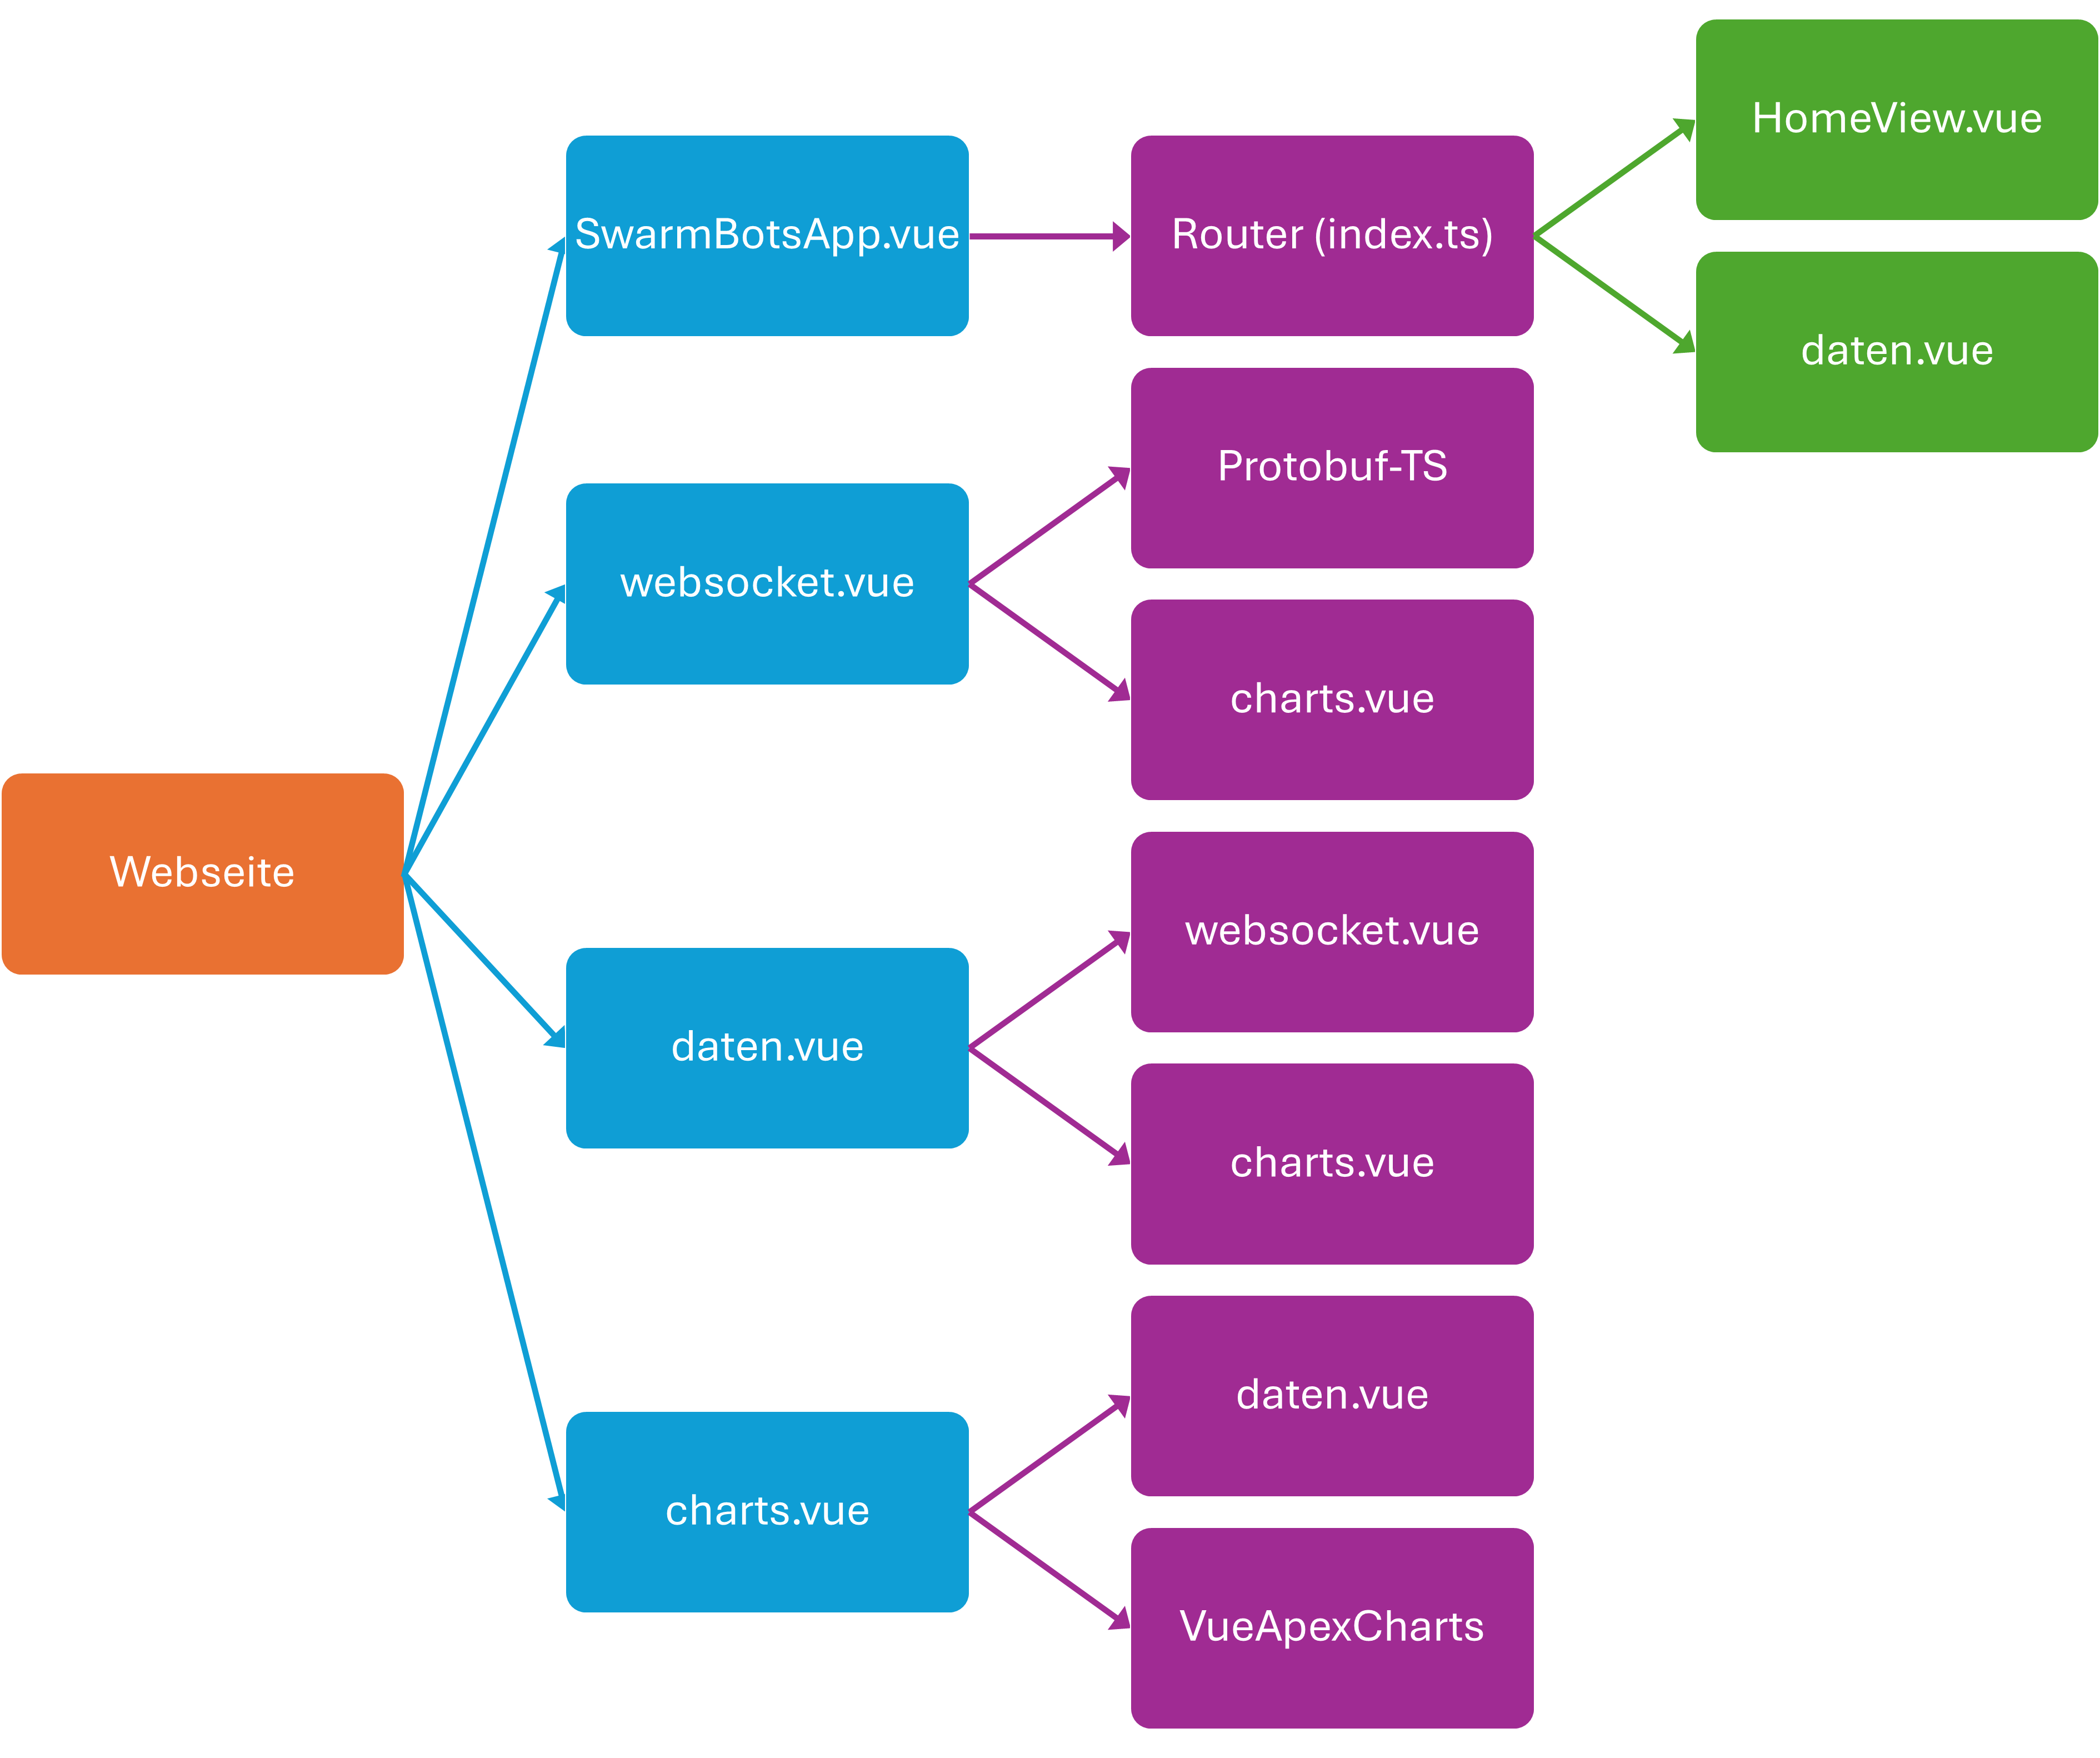
\includegraphics[width=\textwidth, center]{img/Webseite_FD.png}
  \caption{Webseite - Flussdiagramm}
  \label{fig:Webseite_Flowchart}
\end{figure}

\subsection{Webseite - Startseite}
\label{subsubsec:Webseite_Startseite}

\begin{figure}[H]
  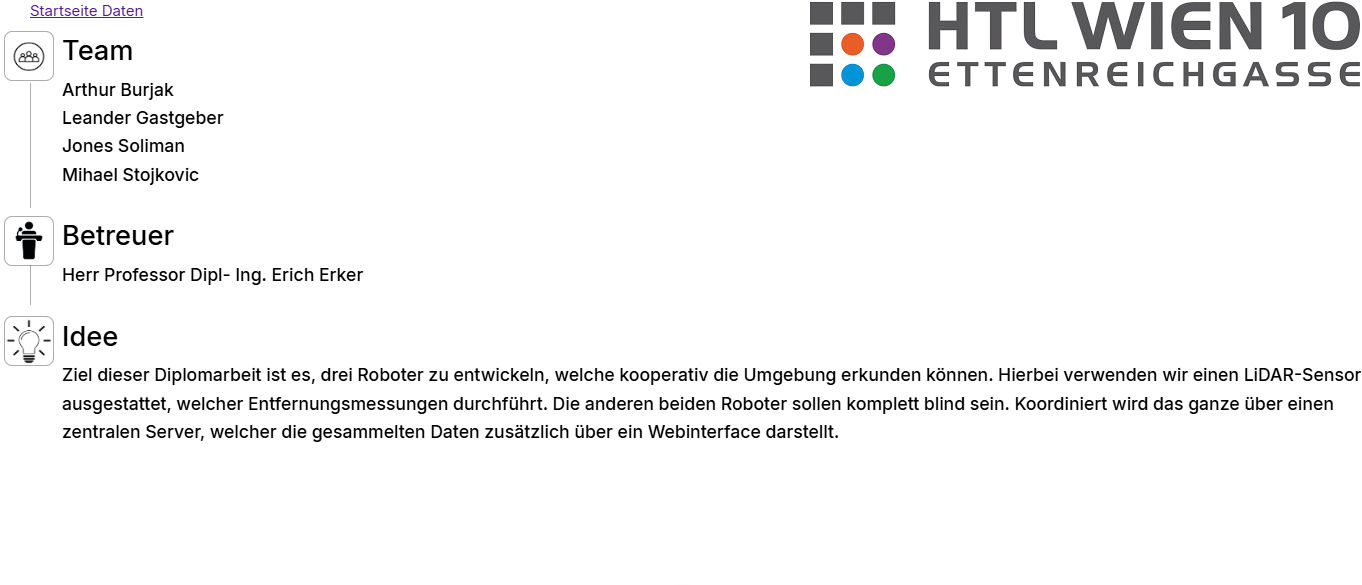
\includegraphics[width=\textwidth, center]{img/Webseite_Startseite.png}
  \caption{Webseite - Startseite}
  \label{fig:Webseite_Startseite}
\end{figure}

Zu sehen ist die fertige Startseite der Diplomarbeitsgruppe ``SwarmBots''. 
Die Umsetzung der Benutzeroberfläche erfolgt unter Verwendung von CSS im Hauptmodul ``SwarmBotsApp.vue''.
%
Das Hauptmodul ``SwarmBotsApp.vue'' beinhaltete ursprünglich alle Komponenten, wurde jedoch im Laufe des Projektes
auf den derzeitigen Stand aufgeteilt um einen bessern Überblick zu gewährleisten.
%
Das Hauptmodul dient derzeitig nur für die Formatierung der Startseite, die auslesung, verarbeitung 
sowie Veranschaulichung der Sensordaten werden in den einzelnen Komponenten erledigt. 
%
Die Startseite bietet dem Nutzer einen übersichtlichen Einstieg in das Projekt. Sie stellt die Mitglieder des Teams
sowie den zuständigen Betreuer vor und vermittelt einen ersten Eindruck der Diplomarbeit. \\
% 
Die Startseite erfüllt zwei wichtige Punkte: Der erste, sie soll dem Nutzer als Informationsquelle der 
Diplomarbeit dienen sowie über ihrer Gruppenmitglieder und ihrem Betreuer. 
Der zweite wesentliche Punkt der Startseite ist es die Navigationslinks anzuzeigen um zu den 
gesammelten Sensordaten zu kommen. 

\subsection{Webseite - Daten}
\label{subsubsec:Webseite_Daten}

\begin{figure}[H]
  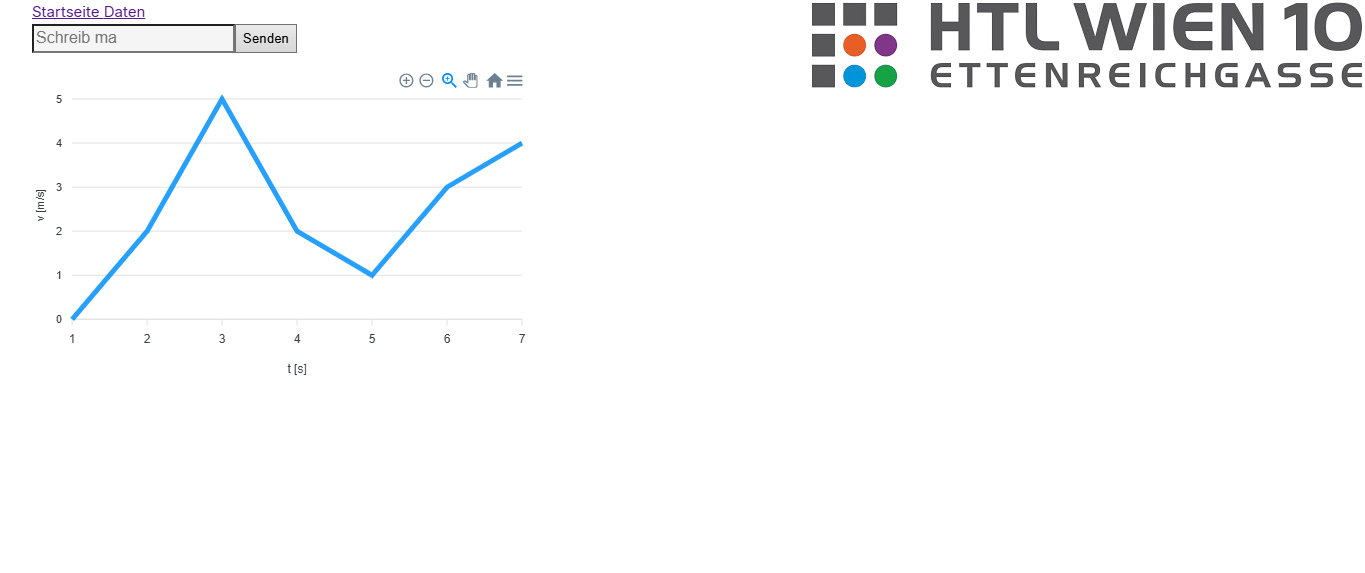
\includegraphics[width=\textwidth, center]{img/Webseite_Daten.png}
  \caption{Webseite - Daten}
  \label{fig:Webseite_Daten}
\end{figure}

Dieser Teil der Webseite ist für die Darstellung sämtlicher emfpangener Daten verantwortlich.
Die empfangenen Daten der Sensoren werden grafisch visualisiert und dem Nutzer in beschrifteten Diagrammen dargestellt. 
%
Zusätzlich neben der vielen gesammelten Sensordaten, wurde ein Websocket integriert, 
der eine zweiseitge Kommunikation mit dem Server ermöglicht. 
%
Die bereitstehende Websocket verbindung dient zur schriftlichen Kommunikation mit dem Server bei etwaigen problemen.
%
Dieser Abschnitt der Webseite ist Aufgrund der Datenvisualisierung der wichtigste im Bereich des Frontends.

\section{LiDAR-Karte}
\label{subsec:frontend_lidar_map}
Die LiDAR-Karte wird im Frontend mithilfe von Vue.js generiert und in stetig aktualisert. 
Die Karte dient der Darstellung von Hindernissen in der Umgebung und zeigt Objekte wie Wände, 
Säulen oder auch Personen in Form von Punktwolken an. 
%
Der LiDAR-Sensor bietet leider keine detaillierte Darstellung der Punktwolke, 
weshalb das Herauslesen unterschiedlicher Hindernisse in manchen Fällen zu Schwierigkeiten führt. 
%
Die Karte soll außerdem zwischen einem Hinderniss sowie den Robotern ``Tamerlan'' und ``Bambi'' 
unterscheiden und diese Hervorheben. 
%
Jedoch sollen nicht nur Hindernisse grafisch dargestellt werden, 
sondern auch die aktuellen Positionen der SwarmBots.
%
Das auslesen der Position der SwarmBots ermgöglicht dem Nutzer mögliche Probleme zu erkennen, 
z.B. wenn die SwarmBots probleme beim erkennen einiger Objekte haben sollten.  

\begin{figure}[H]
    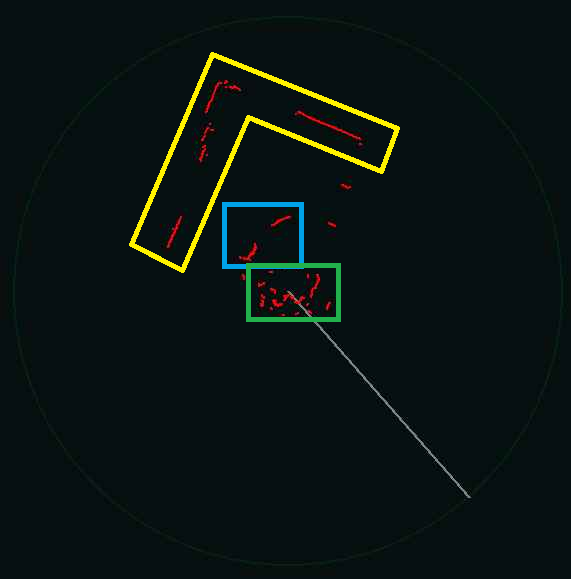
\includegraphics[width=0.7\textwidth, center]{img/LiDARMessungZeichnung_alt.png}
    \caption{LiDAR-Messung}
    \label{fig:LiDAR-Messung}
\end{figure}

Das Bild zeigt die generierte Punktwolke des LiDAR-Sensors.
%
Die Punktwolke zeigt ideal die Funktionsweise des LiDARs
und ist leicht zu interpretieren.
%
Die unterschiedlichen Laserimpulse,
welche gesendet werden,
reflektieren an der Oberfläche und werden gemessen.

Zur einfacheren Interpretation des Beispiels
wurden von Herrn Burjak Bereiche eingezeichnet:
%
Der grüne Bereich zeigt Objekte,
welche unmittelbar vor dem LiDAR standen.
%
In dem Fall waren es Büromaterialien wie etwa Kugelschreiber, Hefte, etc.
%
Blau markiert ist eine Person (links),
die ungefähr in 2.5 m Entfernung vom Sensor
neben einem Sessel (rechts) steht.
%
Im gelbem ``L'' kann man die Wände bzw. Bücherregale erkennen,
welche den Testraum abgegrenzt haben.
Die beiden großen Lücken im gelbem Bereich wurden
durch die Hindernisse im blauem Bereich verursacht,
an denen der Laser bereits schon frühzeitig abgeprallt ist.
%
Die beiden nicht markierten Punkte-``Cluster'' stellen Dachstützen dar.

\section{Anzeigen der Sensordaten}
\label{subsec:frontend_sensors}
Die Sensordaten werden alle auf dem Frontend dargestellt und stetig aktualisiert.
%
Jeder Tumbller-Roboter ist ab Werk mit Beschleunigungssensoren und Drehgebern ausgerüstet,
welche wir gleich für unsere Zwecke wiederverwendet haben.
%
Als Modifikationen haben wir jedem Roboter ein Kompass-Modul
und Guide zusätzlich noch den LiDAR installiert.
%
Der LiDAR erstellt eine Karte in Form einer Punktwolke,
um eventuelle Hindernisse erkennen zu können.
%
Für mehr Informationen zum LiDAR-Sensor siehe Abschnitt \ref{subsec:ueberblick_lidar} oder \ref{subsec:frontend_lidar_map}.

\begin{figure}[H]
    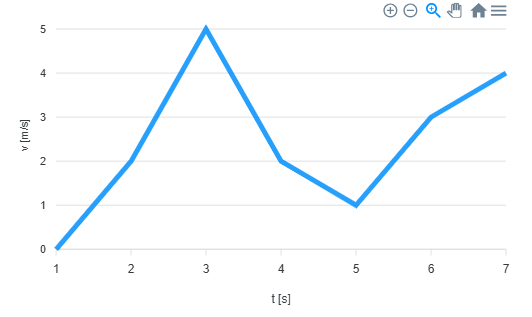
\includegraphics[width=0.8\textwidth, center]{img/encoder_chart.png}
    \caption{Diagramm der Encoderdaten}
    \label{fig:Encoderdaten}
\end{figure}

Die Werte der Beschleunigungssensoren werden,
im Graphen abhängig von der Zeit angezeigt, 
um die aktuellen Werte mit der Vergangenheit vergleichen zu können.

\section{Fernüberwachung per Kamera}
\label{subsec:frontend_cam_stream}
Auf allen drei Robotern befinden sich fest montierte
\texttt{ESP32-CAM}-Kameramodule zur Überwachung,
welche dem Frontend via MJPEG ein Live-Bild bereitstellen.
%
Die Kameras dienen vor allem der Überwachung der Roboter und sollen der Gruppe nur helfen,
mögliche Probleme (z.B. Stiegen) rasch zu identifizieren,
um die Sicherheit der Roboter zu gewährleisten.
%
Eingriffe erfolgen nur falls die Roboter nicht selbstständig erfolgreich die Gefahrensituation vermeiden.
%
Sollte ein Fehler bei der autonomen Steuerung von einem der Roboter aufgetreten sein,
helfen uns die Kameras zusätzlich bei der manuellen Fernsteuerung.
%
So können wir mithilfe der Fernsteuerung (Siehe Abschnitt \ref{subsec:frontend_control}) probieren,
die Roboter z.B. aus einer Gefahrenzone zu entfernen.

\section{Fernsteuerung}
\label{subsec:frontend_control}
Das Konzept der Fernsteuerung wurde aus den Prototypen der Projektwoche aus dem Jahr 2023/2024 übernommen.
%
Diese hatten eine Fernsteuerungsfunktion per Playstation 4 Controller. Einfachkeitshalber wurden die Roboter über 
den Laptop mittels Playstation 4-Controller angesteuert. 
%
Das größte Problem der Playstation 4-Controller besteht darin, dass sie jedes mal ihre MAC-Adresse ändern sofern
man sie über die Roboter verbindet.  
%
Die Fernsteuerungsfunktion sollte aber nur zu Testzwecken dienen um die Roboter 
vor potentiellen Gefahrensituation zu Retten. 

\section{Frontend - Code}
\label{subsec:frontend_Code}
In diesem Kapitel wird sich hauptsächlich auf die Beschreibung der verschiedenen Module des
Frontend-Codes konzentriert. Die Struktur und Funktionalität werden mit der \texttt{``4+1 architectural view model''} beschrieben.
%
Diese Methode wird häufig bei Softwarelastigen Projekten eingesetzt, um komplexe Systeme aus unterschiedlichen
Perspektiven verständlich darzustellen.
Das 4+1 architectural view model kombiniert die fünf Sichten:
\begin{itemize}
  \item Logische Sichte
  \item Entwicklungssicht
  \item Prozesssicht
  \item Physische Sicht
  \item Szenarien
\end{itemize} 
Der Einsatz des Modells hilft bei der Beschreibung Frontend-Codes. 
Dabei wird der Code nicht nur auf seine technische Umsetzung beschreiben,
sondern auch auf seine Funktion im Gesamtsystem 
sowie seiner Abhängigkeit und interaktion mit anderen Komponenten des Projektes.

\subsection{Protobufs generieren - TypeScript}
\label{subsec:proto_gen_TS}
Bevor die Struktur sowie verhaltensweise der Codes genauer erläutert wird,
müssen die Protobufs generiert werden. 
%
Die Webseite benutzt die generierten Protobufs als TypeScript, 
um die notwendigen Daten herauslesen zu können.
%
Nach der Erklärung in \ref{subsec:ueberblick_protobufs} wieso wir Protobufs verwenden,
geht dieses Kapitel genauer drauf ein wie diese generiert werden.
%
Am Anfang der Diplomarbeit wurde die Protobuf-Datein immer händisch generiert, 
nach einiger Zeit war dies zu nervig, weshalb die generierung mit einem Script automatisiert wurde.
%
Das Script wird ausgeführt, sobald die Webseite gebuilted oder gestarted wird.
Dabei hat das Script immer die höhere Priorität, wodurch der Code nur mit den neusten generierten 
TypeScript Dateien arbeitet.
%
Der wesentliche Teil der generierung sieht wie folgt aus:
\begin{lstlisting}[language=JavaScript, gobble=4]
  {
    exec("npx protoc --proto_path=../proto --ts_out=./src/lib/ ../proto/*.proto", (error, stdout, stderr) => {
            if (error)
              console.error('\n'+error.message)
            if (stderr)
              console.error('\n'+stderr)
            if (stdout)
              console.log('\n'+stdout)
        })
        console.log("Compiled protobufs!")
  }
\end{lstlisting}
Die Funktion führt den Befehl zum erstellen der Protobufs sofort aus und speichert sie im Ordner ``lib'',
wo die generierten Protobuf Datein gelagert werden.

\subsection{websocket.vue}
\label{subsec:frontend_websocket.vue}

Bevor die genauer Erklärung bezüglich des websockets.vue Codes kommt,
folgt ein Flussdiagramm, das erstmals die Funktionen und einzelnen Schritte
des Codes beschreibt.
%
Das Flussdiagramm zeigt perfekt die einzelnen Schritte, 
die der Code durcharbeitet um die Geschwindigkeit der Encoder herauszufinden.
Über das Flussdiagramm ist ebenso zu sehen, 
dass der Websocket die Werte für die Diagramme aktualisert. 
%

\begin{figure}[H]
  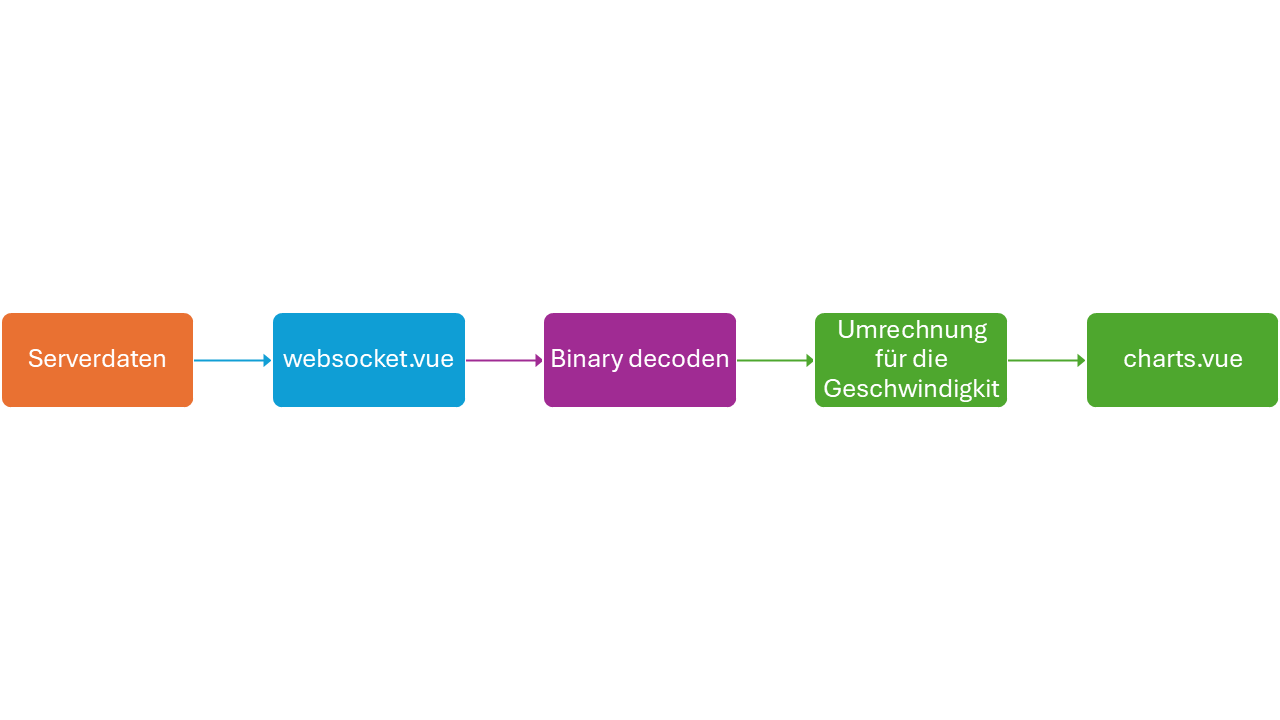
\includegraphics[width=\textwidth, height=13cm, center]{img/Websocket_FD.png}
  \caption{websocket.vue - Flussdiagramm}
  \label{fig:websocket_Flowchart}
\end{figure}

\begin{enumerate}
  \item \texttt{Logische Sicht:} \\
  In der logischen Sicht des 4+1 architectural view models ist das Websocket eine esenzielle Komponente.
  Diese Komponente übernimmt die Kommunikation mit dem Server und verarbeitet die empfangenen Daten.
  Die Komponente deserialisiert diese Daten wodurch sie lesbar werden. Nach der Verarbeitung werden die Daten an 
  eine weitere Komponente (charts.vue) gesendet um grafisch dargestellt werden zu können.
  \item \texttt{Entwicklungssicht:} \\
  Aus der Entwicklersicht ist die Komponente ziemlich fortschrittlich.
  Es wird eine aktuelle Version von Vue verwendet (3.5.13), sowie die neuere Composition-API in Kombination mit TypeScript.
  Dadurch das die vielzahl an Komponenten alle aufgeteilt worden sind,
  ist die Fehlersuche sowie die potenzielle Erweiterung des Codes leicht.
  \item \texttt{Prozesssicht:} \\
  Die Kommunikation erfolgt hauptsächlich Eventgesteuert. 
  Beim Eintreffen neuer Daten vom Server, erscheinen sie direkt auf der Grafik, 
  welche dann unter dem Navigationslink ``Daten'' einzusehen sind. 
  Das Empfangen der Daten erfolgt in Echtzeit, so dass die Seite nicht neugeladen werden muss, 
  außerdem werden alte Daten aus der Grafik entfernt und durch neue ersetzt.
  \item \texttt{Physische Sicht:} \\
  Die Webseite welche mittels dem Vue-Framework geschrieben worden ist läuft nur im Browser.
  Die notwendigen Server- oder Websocket Verbindungen werden automatisch beim Start der Webseite ausgeführt.
  \item \texttt{Szenarien:} \\
    \begin{itemize}
      \renewcommand{\labelitemi}{$\Rightarrow$}
    \item Der Nutzer öffnet die Webseite.
    \item Der Nutzer wechselt auf den Reiter ``Daten'' über die Navigationsleiste.
    \item Der Nutzer bekommt einen Einblick auf alle derzeitig erfassten Daten der Roboter grafisch dargestellt.
    \end{itemize}
\end{enumerate}

\subsection{daten.vue}
\label{subsec:frontend_daten.vue}
Der Code ``daten.vue'' ist im prinzip nahezu der gleiche wie der von \ref{subsec:frontend_websocket.vue}.
Daten.vue unterscheidet sich vor allem darin, dass dieser Code,
nur eine Kommunikation zwischen User und Server durch den Websocket ermöglicht.
%

\subsection{charts.vue}
\label{subsec:frontend_charts.vue}
Beim Code ``charts.vue'', werden die Charts der unterschiedlichen Sensoren erstellt.
%
Der Code ermöglicht eine leichte Ergänzung mehrerer Diagramme und bietet dabei einen guten Überblick.
%



\subsection{SwarmBotsApp.vue}
\label{subsec:frontend_SwarmBotsApp.vue}
TODO

\section{Webseitenprobleme}
\label{subsec:problem_Webseite}
TODO

\subsection{Pfadfindung}
\label{subsubsec:problem_Pfadfindung}
Um bei Vue.js Module zu importieren muss die Funktion \texttt{Import from 'PFAD'} verwendet werden.
%
Um die Encoder Daten welche vom Server geschickt werden verarbeiten zu können, 
müssen erstmals die generierten Protobufdateien gefunden werden.
%
\begin{lstlisting}[language=JavaScript,gobble=4]
  {
    import { EncoderData } from  '../lib/encoder_data'
    ...
    const decodedData = EncoderData.fromBinary(binaryData);
    ...
  }
\end{lstlisting}
Es sollte ``EncoderData`` aus der generierten TypeScript-Protobuf Datei gelesen werden und im Modul ``websocket.vue'' verwendet werden.
Dieser Ansatz wie er oben steht, führt jedoch dazu, dass der Pfad nicht gefunden wird. 
%
Nach viel Recherche viel auf, dass nicht nur JavaScript dateien generiert werden müssen, sondern auch TypeScript Dateien.
Sobald die benötigte TypeScript Datei hinzugefügt wurde, verschwand die Fehlermeldung.
%
Nachdem die vorherigen Fehlermeldungen beseitigt worden waren, kam eine neue auf. 
Der Fehler lag, daran, dass die neuen generierten Files das "google-Protobuf" Packet brauchten um zu funktionieren.
% 
\begin{lstlisting}[language=JavaScript,gobble=4]
  {
    import * as pb_1 from "google-protobuf";
    ...
  }
\end{lstlisting}
Dies war leicht zu beheben mit dem Befehl:\\ \texttt{npm install -D @types/google-protobuf} \\ wurden die Packete schnell
heruntergeladen.

\subsection{Variablen einlesung}
\label{subsubsec:problem_variablen_einlesen}

Ein hartnäckiges Problem war das einlesen der Variablen von den Protobufs. 
%
Nachdem der TypeScript-Protobuf nun korrekt eingelesen wird, 
musste dieser natürlich auch sofort getestet werden.
%
Der Code wurde geschrieben und die Variablen die in der Protobuf-Datei verarbeiten werden, 
sollten wie folgt eingelesen eingelesen werden.
\begin{lstlisting}[language=JavaScript, gobble=4]
  {
    const pulses = data.pulses;
    const duration = data.duration;
  }
\end{lstlisting}

Es wurde mehrere Male überprüft, ob nun wirklich die notwendigen Daten wirklich über die Variable 
``data.pulses'' und ``data.duration'' geschickt werden. 
%
Trotz der Überprüfung der Schüler ob der Code korrekt ist, 
trotz Recherche im Internet und befragungen an den Lehrpersonen, konnte kein Fehler klargestellt werden.
%
Nachdem wir als Gruppe nahezu fast jeden erdenklichen Schritt durchgegangen sind, um diesen Fehler zu beheben,
kamen wir als Gruppe auf den Gedanken, die Protobuf-Files mal neu generieren zu lassen, da möglicherweise 
%
die erstellten Codes Fehler beinhlten konnten. 
%
Nachdem die TypeScript Datei neu erstellt worden ist (Für den Befehl siehe \ref{subsec:proto_gen_TS}),
wurde der Code der generation geändert, weshalb die Variablen nun anders einglesen werden müssen,
um die korrekten Werte zu erhalten.
%
die neue Änderung sieht wie folgt aus:
\begin{lstlisting}[language=JavaScript, gobble=4]
  {
    const decodedData = EncoderData.fromBinary(binaryData);

    const pulses = decodedData.pulses;
    const duration = decodedData.duration;
    ...
  }
\end{lstlisting}
Der neue Code speichert beide Werte, also data.pulses und data.duration in ``EncoderData''.
EncoderData wird ausgelesen und als ``decodedData'' gespeichert, davon werden die benötigten Werte
dann rausgelesen und weitergeschickt.

\subsection{Diagramm anzeigen}
\label{subsubsec:problem_chart_anzeige}

Ein lästiges Problem was zum Glück jedoch nicht lange anhielt, war das Problem die Diagramme anzeigen zu lassen.
Hier spielte wieder die Pfadfindung (siehe \ref{subsubsec:problem_Pfadfindung} für mehr Infos) ein Problem.
%
Neben der erneuten Pfadfindungs probleme, kam ein neues Problem auf. 
Leider wurden im Code ``websocket.vue'', das Diagramm nicht korrekt einglesen über den Befehl
\begin{lstlisting}[language=JavaScript, gobble=4]
  {
    export default {
      name: "Websocket",
      components: {
        encoder_Chart,
      },
    }
  }
\end{lstlisting}
Hierbei handelte es sich um einen klassisches ``Copy \& Paste'' Fehler, da diese Code Zeile aus dem Code
``charts.vue'' herauskopiert wurde.
%

\subsection{Build-Probleme}
\label{subsubsec:problem_Builden}

Am anfang der Diplomarbeit begann jeder seine Arbeit lokal auf dem eigenen PC.
%
Nach einiger Zeit mussten die Codes aber auf Github hochgeladen werden für einen besseren Überblick 
des Fortschrittes der Diplomarbeitsgruppe und damit der Betreuer der Gruppe jederzeit den Fortschritt 
seiner Gruppe sich anschauen kann. 
%
Das erste mal Hochladen des Codes auf Github führte direkt zu Problemen, 
da der Code lokal auf dem PC wunderbar lief und Funktionierte, 
jedoch sobald er auf Github hochgeladen worden ist, 
Der Code nicht mehr Compilen bzw. builden wollte.
%
Diese Problem konnte jedoch durch eine kleine Bedenktzeit schnell gelöst werden,
da Irrtümlicherweise vergessen im entsprechenden Ordner zu arbeiten.
%
Das große Problem dabei ist, dass die notwendigen Funktionen von Vue nur im entsprechenden Ordner zugänglich sind.
%
